\vspace{3cm}

$\hphantom{aaaaaaa}$

\begin{center}
    \bf 
Quantili della distribuzione t di Student con $\nu$ gradi di libertà
\[
    F_{\nu}(t) = \int_{-\infty}^t \frac{\Gamma[\frac{\nu+1}{2}]}{\sqrt{\nu\pi} \: \Gamma[\frac{\nu}{2}] \: \left(1+\frac{t^2}{\nu} \right)^{\frac{\nu+1}{2}}} \, dt
\]
\end{center}

\begin{center}
    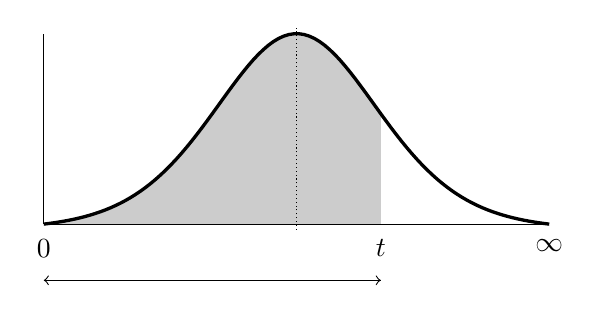
\begin{tikzpicture}[
    declare function={gamma(\z)=
    2.506628274631*sqrt(1/\z)+ 0.20888568*(1/\z)^(1.5)+ 0.00870357*(1/\z)^(2.5)- (174.2106599*(1/\z)^(3.5))/25920- (715.6423511*(1/\z)^(4.5))/1244160)*exp((-ln(1/\z)-1)*\z;},
    declare function={student(\x,\n)= gamma((\n+1)/2.)/(sqrt(\n*pi) *gamma(\n/2.)) *((1+(\x*\x)/\n)^(-(\n+1)/2.));}
]
        \begin{axis}[
                no markers, domain=-3:3, samples=100,
                axis lines*=left, %xlabel=$x$, ylabel=$y$,
                height=4cm, width=8cm,
                xtick=\empty, ytick=\empty,
                enlargelimits=false, clip=false, axis on top,
                grid = major
            ]
            \addplot [fill=black!20, draw=none, domain=-3:1] {student(x,10)} \closedcycle;
            \addplot [very thick,black!50!black] {student(x,10)};
            
            \node[below] at (axis cs: -3, 0)  {$0$};
            \node[below] at (axis cs: 1, 0)  {$t$};
            \node[below] at (axis cs: 3, 0) {$\infty$};
            \draw[-, densely dotted] (axis cs: 0, 0) -- (axis cs: 0, 0.4);
            \draw[->] (axis cs: 1, -0.1) -- (axis cs: -3, -0.1);            
            \draw[->] (axis cs: -3, -0.1) -- (axis cs: 1, -0.1);
        \end{axis}
    \end{tikzpicture}
\end{center}

\begin{table}[ht]
\centering
\begin{tabular}{rrrrrrrrrrr}
  \hline
 & \textbf{0.6} & \textbf{0.75} & \textbf{0.9} & \textbf{0.95} & \textbf{0.975} & \textbf{0.99} & \textbf{0.995} & \textbf{0.9975} & \textbf{0.999} & \textbf{0.9995} \\
  \hline
  \textbf{1 } & 0.3249 & 1.0000 & 3.0777 & 6.3138 & 12.7062 & 31.8205 & 63.6567 & 127.3213 & 318.3088 & 636.6192 \\
  \textbf{2 } & 0.2887 & 0.8165 & 1.8856 & 2.9200 & 4.3027 & 6.9646 & 9.9248 & 14.0890 & 22.3271 & 31.5991 \\
  \textbf{3 } & 0.2767 & 0.7649 & 1.6377 & 2.3534 & 3.1824 & 4.5407 & 5.8409 & 7.4533 & 10.2145 & 12.9240 \\
  \textbf{4 } & 0.2707 & 0.7407 & 1.5332 & 2.1318 & 2.7764 & 3.7469 & 4.6041 & 5.5976 & 7.1732 & 8.6103 \\
  \textbf{5 } & 0.2672 & 0.7267 & 1.4759 & 2.0150 & 2.5706 & 3.3649 & 4.0321 & 4.7733 & 5.8934 & 6.8688 \\
  \textbf{6 } & 0.2648 & 0.7176 & 1.4398 & 1.9432 & 2.4469 & 3.1427 & 3.7074 & 4.3168 & 5.2076 & 5.9588 \\
  \textbf{7 } & 0.2632 & 0.7111 & 1.4149 & 1.8946 & 2.3646 & 2.9980 & 3.4995 & 4.0293 & 4.7853 & 5.4079 \\
  \textbf{8 } & 0.2619 & 0.7064 & 1.3968 & 1.8595 & 2.3060 & 2.8965 & 3.3554 & 3.8325 & 4.5008 & 5.0413 \\
  \textbf{9 } & 0.2610 & 0.7027 & 1.3830 & 1.8331 & 2.2622 & 2.8214 & 3.2498 & 3.6897 & 4.2968 & 4.7809 \\
  \textbf{10} & 0.2602 & 0.6998 & 1.3722 & 1.8125 & 2.2281 & 2.7638 & 3.1693 & 3.5814 & 4.1437 & 4.5869 \\
  \textbf{11} & 0.2596 & 0.6974 & 1.3634 & 1.7959 & 2.2010 & 2.7181 & 3.1058 & 3.4966 & 4.0247 & 4.4370 \\
  \textbf{12} & 0.2590 & 0.6955 & 1.3562 & 1.7823 & 2.1788 & 2.6810 & 3.0545 & 3.4284 & 3.9296 & 4.3178 \\
  \textbf{13} & 0.2586 & 0.6938 & 1.3502 & 1.7709 & 2.1604 & 2.6503 & 3.0123 & 3.3725 & 3.8520 & 4.2208 \\
  \textbf{14} & 0.2582 & 0.6924 & 1.3450 & 1.7613 & 2.1448 & 2.6245 & 2.9768 & 3.3257 & 3.7874 & 4.1405 \\
  \textbf{15} & 0.2579 & 0.6912 & 1.3406 & 1.7531 & 2.1314 & 2.6025 & 2.9467 & 3.2860 & 3.7328 & 4.0728 \\
  \textbf{16} & 0.2576 & 0.6901 & 1.3368 & 1.7459 & 2.1199 & 2.5835 & 2.9208 & 3.2520 & 3.6862 & 4.0150 \\
  \textbf{17} & 0.2573 & 0.6892 & 1.3334 & 1.7396 & 2.1098 & 2.5669 & 2.8982 & 3.2224 & 3.6458 & 3.9651 \\
  \textbf{18} & 0.2571 & 0.6884 & 1.3304 & 1.7341 & 2.1009 & 2.5524 & 2.8784 & 3.1966 & 3.6105 & 3.9216 \\
  \textbf{19} & 0.2569 & 0.6876 & 1.3277 & 1.7291 & 2.0930 & 2.5395 & 2.8609 & 3.1737 & 3.5794 & 3.8834 \\
  \textbf{20} & 0.2567 & 0.6870 & 1.3253 & 1.7247 & 2.0860 & 2.5280 & 2.8453 & 3.1534 & 3.5518 & 3.8495 \\
  \textbf{21} & 0.2566 & 0.6864 & 1.3232 & 1.7207 & 2.0796 & 2.5176 & 2.8314 & 3.1352 & 3.5272 & 3.8193 \\
  \textbf{22} & 0.2564 & 0.6858 & 1.3212 & 1.7171 & 2.0739 & 2.5083 & 2.8188 & 3.1188 & 3.5050 & 3.7921 \\
  \textbf{23} & 0.2563 & 0.6853 & 1.3195 & 1.7139 & 2.0687 & 2.4999 & 2.8073 & 3.1040 & 3.4850 & 3.7676 \\
  \textbf{24} & 0.2562 & 0.6848 & 1.3178 & 1.7109 & 2.0639 & 2.4922 & 2.7969 & 3.0905 & 3.4668 & 3.7454 \\
  \textbf{25} & 0.2561 & 0.6844 & 1.3163 & 1.7081 & 2.0595 & 2.4851 & 2.7874 & 3.0782 & 3.4502 & 3.7251 \\
  \textbf{26} & 0.2560 & 0.6840 & 1.3150 & 1.7056 & 2.0555 & 2.4786 & 2.7787 & 3.0669 & 3.4350 & 3.7066 \\
  \textbf{27} & 0.2559 & 0.6837 & 1.3137 & 1.7033 & 2.0518 & 2.4727 & 2.7707 & 3.0565 & 3.4210 & 3.6896 \\
  \textbf{28} & 0.2558 & 0.6834 & 1.3125 & 1.7011 & 2.0484 & 2.4671 & 2.7633 & 3.0469 & 3.4082 & 3.6739 \\
  \textbf{29} & 0.2557 & 0.6830 & 1.3114 & 1.6991 & 2.0452 & 2.4620 & 2.7564 & 3.0380 & 3.3962 & 3.6594 \\
  \textbf{30} & 0.2556 & 0.6828 & 1.3104 & 1.6973 & 2.0423 & 2.4573 & 2.7500 & 3.0298 & 3.3852 & 3.6460 \\
  \textbf{50} & 0.2547 & 0.6794 & 1.2987 & 1.6759 & 2.0086 & 2.4033 & 2.6778 & 2.9370 & 3.2614 & 3.4960 \\
  \textbf{75} & 0.2542 & 0.6778 & 1.2929 & 1.6654 & 1.9921 & 2.3771 & 2.6430 & 2.8924 & 3.2025 & 3.4250 \\
  \textbf{100} & 0.2540 & 0.6770 & 1.2901 & 1.6602 & 1.9840 & 2.3642 & 2.6259 & 2.8707 & 3.1737 & 3.3905 \\
  \textbf{$+\infty$} & 0.2533 & 0.6745 & 1.2816 & 1.6449 & 1.9600 & 2.3263 & 2.5758 & 2.8070 & 3.0902 & 3.2905 \\
   \hline
\end{tabular}
\end{table}






